\documentclass{amsart}
\usepackage[margin = 2.5cm]{geometry}
\usepackage{sagetex} % Para usar sagetex
%\usepackage[usefamily=sage]{pythontex} % Para usar pythontex
\usepackage[utf8]{inputenc}
\usepackage{tikz}

\newtheorem{ejer}{Ejercicio}

\title{Álgebra y Matemática Discreta. GII - FIUM. \\ Parcial 1}
\begin{document}
\maketitle


\begin{ejer} 
Calcula el determinante de la siguiente matriz sobre el cuerpo
${\mathbb Z}_5$ realizando operaciones elementales. 
$$ \left|\begin{array}{rrrr}
1 & 0 & 2 & 0 \\
3 & 3 & 2 & 0 \\
3 & 4 & 0 & 4 \\
0 & 2 & 4 & 3
\end{array}\right|$$
{\bf Este problema hay que hacerlo a mano en el papel proporcionado
en el examen.}
\end{ejer}

{\it Solución: }

$$
\left|\begin{array}{rrrr}
	1 & 0 & 2 & 0 \\
	3 & 3 & 2 & 0 \\
	3 & 4 & 0 & 4 \\
	0 & 2 & 4 & 3
\end{array}\right| 
\to E_{(3) - 3(1)}
\left|\begin{array}{rrrr}
	1 & 0 & 2  & 0 \\
	3 & 3 & 2  & 0 \\
	0 & 4 & 4 & 4 \\
	0 & 2 & 4  & 3
\end{array}\right| 
\to E_{(2) - 3(1)}
\left|\begin{array}{rrrr}
	1 & 0 & 2  & 0 \\
	0 & 3 & 1  & 0 \\
	0 & 4 & 4  & 4 \\
	0 & 2 & 4  & 3
\end{array}\right| 
\to E_{(3) - 2(4)}
\left|\begin{array}{rrrr}
	1 & 0 & 2 & 0 \\
	0 & 3 & 1 & 0 \\
	0 & 0 & 1 & 3 \\
	0 & 2 & 4 & 3
\end{array}\right|
$$
$$
\to E_{(2) - (4)}
\left|\begin{array}{rrrr}
	1 & 0 & 2 & 0 \\
	0 & 1 & 2 & 2 \\
	0 & 0 & 1 & 3 \\
	0 & 2 & 4 & 3
\end{array}\right| 
\to E_{(4) - 2(2)}
\left|\begin{array}{rrrr}
	1 & 0 & 2 & 0 \\
	0 & 1 & 2 & 2 \\
	0 & 0 & 1 & 3 \\
	0 & 0 & 0 & 4
\end{array}\right| 
\to E_{(1) - 2(3)}
\left|\begin{array}{rrrr}
	1 & 0 & 0 & 4 \\
	0 & 1 & 2 & 2 \\
	0 & 0 & 1 & 3 \\
	0 & 0 & 0 & 4
\end{array}\right| 
\to E_{(4) - (1)}
\left|\begin{array}{rrrr}
	1 & 0 & 0 & 4 \\
	0 & 1 & 2 & 2 \\
	0 & 0 & 1 & 3 \\
	4 & 0 & 0 & 0
\end{array}\right| 
$$
$$
\to E_{(4) - 4(1)}
\left|\begin{array}{rrrr}
	1 & 0 & 0 & 4 \\
	0 & 1 & 2 & 2 \\
	0 & 0 & 1 & 3 \\
	0 & 0 & 0 & 1
\end{array}\right| 
\to E_{(3) - 3(4)}
\left|\begin{array}{rrrr}
	1 & 0 & 0 & 4 \\
	0 & 1 & 2 & 2 \\
	0 & 0 & 1 & 0 \\
	0 & 0 & 0 & 1
\end{array}\right| 
\to E_{(2) - 2(4)}
\left|\begin{array}{rrrr}
	1 & 0 & 0 & 4 \\
	0 & 1 & 2 & 0 \\
	0 & 0 & 1 & 0 \\
	0 & 0 & 0 & 1
\end{array}\right| 
\to E_{(2) - 2(3)}
\left|\begin{array}{rrrr}
	1 & 0 & 0 & 4 \\
	0 & 1 & 0 & 0 \\
	0 & 0 & 1 & 0 \\
	0 & 0 & 0 & 1
\end{array}\right| 
$$
$$
\to E_{(1) - 4(4)}
\left|\begin{array}{rrrr}
	1 & 0 & 0 & 0 \\
	0 & 1 & 0 & 0 \\
	0 & 0 & 1 & 0 \\
	0 & 0 & 0 & 1
\end{array}\right| 
= 1
$$

\vspace{10cm}

\begin{ejer}
Encuentra todos los valores enteros $n$ que cumplan 
simultáneamente las siguientes condiciones:
\begin{align*}
n & \equiv 1 \pmod{25} \\
n & \equiv 52 \pmod{108} \\
n & \equiv 199 \pmod{201} 
\end{align*}
\end{ejer}

{\it Solución: }

% Escribe tu solución para el Ejercicio 2

% Fin del ejercicio 2

\begin{ejer}
Sea $K = {\mathbb Z}_{43}$ y $f:K^4 \to K^3$ la aplicación lineal
dada por la matriz $$M(f) = \left(\begin{array}{rrrr}
24 & 23 & 11 & 26 \\
9 & 17 & 33 & 22 \\
16 & 16 & 13 & 4
\end{array}\right)$$
Encuentra dos aplicaciones lineales diferentes $g_1,g_2:K^3 \to K^4$ 
tales que $f\circ g_1 = {\sf id}_{K^3} = f\circ g_2$.
\end{ejer}

{\it Solución: }

% Escribe tu solución para el Ejercicio 3

% Fin del ejercicio 3

\begin{ejer}
Sea $K = {\mathbb Z}_{7}$ y consideremos las bases de $K^3$ dadas por
$ B_1 = \{v_1,v_2,v_3\}$ y $B_2 = \{w_1,w_2,w_3\}$
siendo 
$$
v_1 = \left(\begin{array}{r}
0 \\
0 \\
5
\end{array}\right) \quad 
v_2 = \left(\begin{array}{r}
1 \\
0 \\
0
\end{array}\right) \quad
v_3 = \left(\begin{array}{r}
5 \\
5 \\
5
\end{array}\right)
\quad
w_1 = \left(\begin{array}{r}
4 \\
0 \\
1
\end{array}\right) \quad
w_2 = \left(\begin{array}{r}
3 \\
1 \\
1
\end{array}\right) \quad
w_3 = \left(\begin{array}{r}
2 \\
5 \\
2
\end{array}\right)
$$
Dado el vector $v = \left(\begin{array}{r}
0 \\
1 \\
2
\end{array}\right)_B$, responde a las siguientes preguntas:
\begin{itemize}
\item Calcula la matriz de cambio de base $B$ a la base canónica.
\item Utiliza la matriz anterior para calcular las coordenadas de
$v$ en base canónica.
\item Calcula la matriz de cambio de base $B$ a $B'$.
\item Utiliza la matriz anterior para calcular las coordenadas de
$v$ en base $B'$.
\item Determina si los vectores $\{w_1,w_2,v\}$ forman una base
de $K^3$.
\end{itemize}
\end{ejer}

{\it Solución: }

% Escribe tu solución para el Ejercicio 4

% Fin del ejercicio 4

\begin{ejer}
De termina si existe un camino abierto euleriano en el siguiente
grafo. En caso de existir, calcúlalo:

\begin{center}
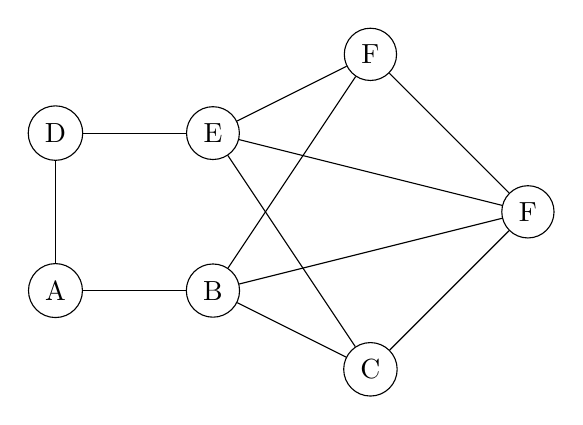
\begin{tikzpicture}[vertice/.style = {fill=white,circle,draw}]
\node[vertice] (A) at (0,0) {A};
\node[vertice] (B) at (2,0) {B};
\node[vertice] (C) at (4,-1) {C};
\node[vertice] (D) at (0,2) {D};
\node[vertice] (E) at (2,2) {E};
\node[vertice] (F) at (4,3) {F};
\node[vertice] (H) at (6,1) {F};

\draw (A) -- (B);
\draw (B) -- (C);
\draw (C) -- (H);
\draw (H) -- (F);
\draw (F) -- (E);
\draw (E) -- (D);
\draw (D) -- (A);
\draw (E) -- (C);
\draw (B) -- (F);
\draw (E) -- (H);
\draw (B) -- (H);
\end{tikzpicture} 
\end{center}
\end{ejer}

{\it Solución: }

% Escribe tu solución para el Ejercicio 5

% Fin del ejercicio 5


\end{document}
